\newpage
\section{CẤP SỐ CỘNG}
\subsection{LÝ THUYẾT CẦN NHỚ}
\subsubsection{Câp số cộng}
\indam{Định nghĩa}
	\begin{boxdn}
	\begin{itemize}
		\item Dãy số $\left(u_n\right)$ là cấp số cộng nếu $u_n=u_{n-1}+d$ với $n\ge 2,d$ là số không đổi.
		\item Số $d$ gọi là công sai của cấp số cộng, $d=u_n-u_{n-1}$ với $n\ge 2$.
		\item Nếu $d=0$ thì cấp số cộng là một dãy số không đổi.
	\end{itemize}	 
	\end{boxdn}
\subsubsection{Số hạng tổng quát}
Cho cấp số cộng $\left(u_n\right)$ có số hạng đầu $u_1$ và công sai $d$, ta có
	\[u_n=u_1+(n-1)d \text{ với } n\ge 2.\] 
\subsubsection{Tổng $n$ số hạng đầu của một cấp số cộng}
	Cho cấp số cộng $\left(u_n\right)$ có số hạng đầu $u_1$ và công sai $d$. Đặt $S_n=u_1+u_2+\ldots +u_n$, ta có:
	\[S_n=\dfrac{\left(u_1+u_n \right)n}{2}\text{ hoặc }S_n=\dfrac{\left[ 2u_1+(n-1)d\right]n}{2}.\]
%-------------------------------------------------------------------------------------------------------------
\subsection{PHÂN LOẠI VÀ PHƯƠNG PHÁP GIẢI TOÁN}
\begin{dang}{Chứng minh một dãy số là cấp số cộng}
	Với dãy số $\left(u_n\right)$, chứng minh hiệu $u_n-u_{n-1}$ không đổi với mọi $n\ge 2$.
\end{dang}
\begin{vd}%[1D2N2-2]
Tìm cấp số cộng trong các dãy số sau
\begin{multicols}{3}
\begin{enumerate}
	\item $1;-3;-7;-11;-15$;
	\item $1;-3;-6;-9;-12$;
	\item $1;-2;-4;-6;-8$.
\end{enumerate}
\end{multicols}
\loigiai{
\begin{enumerate}
	\item Dãy số $1;-3;-7;-11;-15$ là cấp số cộng với công sai $d=-4$.
	\item Ta có $(-3)-1\neq (-6)-(-3)$.\\
	Vậy dãy số $1;-3;-6;-9;-12$ không là cấp số cộng.
	\item Ta có $(-2)-1\neq (-4)-(-2)$.\\
	Vậy dãy số $1;-2;-4;-6;-8$ không là cấp số cộng.
\end{enumerate}
}
\end{vd}

\begin{vd}%[1D2H2-2]
	Trong các dãy số $\left(u_n\right)$ với số hạng tổng quát sau, dãy số nào là cấp số cộng? Nếu là cấp số cộng, hãy tìm số hạng đầu $u_1$ và công sai $d$.
	\begin{enumerate}
	\item $u_n=3-2n$;
	\item $u_n=3^n$.
	\end{enumerate}
	\loigiai{
		\begin{enumerate}
		\item Ta có $u_1=3-2.1=1$; $u_n-u_{n-1}=3-2n-\left[ 3-2\left(n-1\right) \right]=-2$ với mọi $n\ge 2$.\\
		Vậy dãy số $\left(u_n\right)$ đã cho là một cấp số cộng có số hạng đầu $u_1=1$ và công sai $d=-2$.
		\item Ta có $u_1=3$; $u_{2}=9$; $u_{3}=27;\ldots $ Do đó, $u_2-u_1=6$; $u_3-u_2=18$.\\
		Vậy dãy số $\left(u_n\right)$ đã cho không là một cấp số cộng.
		\end{enumerate}	
	}
\end{vd}

\begin{vd}%[1D2H2-1]
Trong các dãy số $\left(u_n\right)$ cho bởi số hạng tổng quát $u_n$ sau, dãy số nào là cấp số cộng? Tìm số hạng đầu và công sai của nó.
\begin{multicols}{2}
	\begin{enumerate}
		\item $u_n=2 n+3$;
		\item $u_n=-3 n+1$;
		\item $u_n=n^2+1$;
		\item $u_n=\dfrac{2}{n}$.
	\end{enumerate}
\end{multicols}

\loigiai{
\begin{enumerate}
	\item Xét hiệu $\begin{aligned}[t]
		u_{n+1}-u_n&=\left[2(n+1)+3\right]-(2n+3)\\
		&=2n+2+3-2n-3\\
		&=2.
	\end{aligned}$\\
	Vậy dãy số đã cho là cấp số cộng, có
	\begin{itemize}
		\item Số hạng đầu $u_1=2\cdot 1+3=5$.
		\item Công sai $d=2$.
	\end{itemize}
	\item Xét hiệu $\begin{aligned}[t]
		u_{n+1}-u_n&=\left[-3(n+1)+1\right]-(-3n+1)\\
		&=-3n-3+1+3n-1\\
		&=-3.
	\end{aligned}$\\
	Vậy dãy số đã cho là cấp số cộng, có
	\begin{itemize}
		\item Số hạng đầu $u_1=-3\cdot 1+1=-2$.
		\item Công sai $d=-3$.
	\end{itemize}
	\item Xét hiệu $\begin{aligned}[t]
	u_{n+1}-u_n&=\left[(n+1)^2+1\right]-(n^2+1)\\
		&=n^2+2n+1+1-n^2-1\\
		&=2n+1.
	\end{aligned}$\\
	Vậy dãy số đã cho không phải là cấp số cộng.
	\item Xét hiệu $\begin{aligned}[t]
		u_{n+1}-u_n&=\dfrac{2}{n+1}-\dfrac{2}{n}\\
		&=\dfrac{2n-2(n+1)}{n(n+1)}\\
		&=\dfrac{2n-2n-2}{n(n+1)}\\
		&=\dfrac{-2}{n(n+1)}.
	\end{aligned}$\\
	Vậy dãy số đã cho không phải là cấp số cộng.
\end{enumerate}
}
\end{vd}

\begin{vd}[Trích đề thi GHKI Trường THPT Nguyễn Thị Minh Khai-TPHCM NH24-25]%[1D2H2-2]%
	Chứng minh dãy số $\left(u_n\right)$ với $u_n=2024n-2025$ là cấp số cộng. Xác định công sai, số hạng đầu của cấp số cộng đó.
	\loigiai{
		Ta có $u_n=2024n-2025\Rightarrow u_{n+1}=2024(n+1)-2025=2024n-1$.\\
		Vì $u_{n+1}-u_n=2024$ nên dãy số $\left(u_n\right)$ là một cấp số cộng với $\heva{&d=2024\\&u_1=-1.}$
	}
\end{vd}

\begin{dang}{Xác định số hạng và công sai của cấp số cộng}
	Áp dụng $u_n=u_1+(n-1)d$ để chuyển các số hạng về $u_1$ và $d$.\\
	Giải phương trình hoặc hệ phương trình để tìm $u_1, d, n,\ldots$
\end{dang}

\begin{vd}%[1D2H2-3]
	Cho cấp số cộng $(u_n)$ có số hạng đầu $u_1=-3$, công sai $d=5$.
	\begin{enumEX}{1}
		\item Viết công thức của số hạng tổng quát $u_n$.
		\item Số $492$ là số hạng thứ mấy của cấp số cộng trên?
		\item Số $300$ có là số hạng nào của cấp số cộng trên không?
	\end{enumEX}
	\loigiai{
		\begin{enumEX}{1}
			\item Ta có $u_n=u_1+(n-1)d=-3+(n-1)\cdot 5=5n-8$.
			\item Ta có $5n-8=492 \Leftrightarrow n=100$. Vậy số $492$ là số hạng thứ $100$ của $(u_n)$.
			\item Nhận thấy $5n-8=300 \Leftrightarrow n=\dfrac{308}{5}=61,6 \notin \mathbb{N}^*$. Vậy số $300$ không là số hạng nào của $(u_n)$.
		\end{enumEX}
	}
\end{vd}

\begin{vd}%[1D2H2-3]
	Tìm số hạng đầu và công sai của cấp số cộng $(u_n)$, biết $u_5=19, u_9=35$.
	\loigiai{
		Gọi $d$ là công sai của CSC, ta có $\heva{&u_5=19\\ &u_9=35}\Leftrightarrow \heva{&u_1+4d=19\\ &u_1+8d=35} \Leftrightarrow \heva{&u_1=3\\ &d=4.}$\\
		Vậy số hạng đầu của cấp số cộng đó là $u_1=3$ và công sai $d=4$.
	}
\end{vd}

\begin{vd}%[1D2H2-3]
	Cho cấp số cộng $(u_n)$ với $u_1=\dfrac{1}{3}$ và $u_1+u_2+u_3=-1$.
	Tìm công sai $d$ và viết công thức của số hạng tổng quát $u_n$.
	\loigiai{
		Ta có $u_1+u_2+u_3=-1$ hay $3 u_1+3 d=-1$. Mà $u_1=\dfrac{1}{3}$ nên $d=-\dfrac{2}{3}$. \\
		Công thức của số hạng tổng quát $u_n$ là $u_n=\dfrac{1}{3}+(n-1)\left(-\dfrac{2}{3}\right)=-\dfrac{2}{3} n+1$.
	}
\end{vd}

\begin{vd}%[1D2H2-3]
	Tìm số hạng đầu $u_1$ và công sai $d$ của cấp số cộng $(u_n)$, biết $\heva{&u_3-u_7=-8\\& u_2\cdot u_7 =75.}$
	\loigiai{
	Áp dụng công thức $u_n=u_1+(n-1)\cdot d$.\\
	Ta có
	\allowdisplaybreaks
		\begin{eqnarray*}
		&&\heva{&u_3-u_7=-8\\& u_2\cdot u_7 =75}\Leftrightarrow \heva{&(u_1+2d)-(u_1+6d)=-8\\& (u_1+d)\cdot (u_1+6d)=75}\Leftrightarrow \heva{&-4d=-8\\& (u_1+d)\cdot (u_1+6d)=75}\\
		&\Leftrightarrow&\heva{&d=2\\& (u_1+2)\cdot (u_1+6\cdot 2)=75}\Leftrightarrow \heva{&d=2\\& u_1^2+14u_1-51=0}\Leftrightarrow \heva{&d=2\\& \hoac{&u_1=3\\& u_1=-17}}\Leftrightarrow \hoac{&\heva{& u_1=3\\& d=2} \\&\heva{&u_1=-17\\&d=2.}}
		\end{eqnarray*}
	Vậy $u_1=3$, $d=2$ hoặc $u_1=-17$, $d=2$.
	}
\end{vd}

\begin{dang}{Tính tổng $n$ số hạng đầu của cấp số cộng}
	Áp dụng $S_n=\dfrac{(u_1+u_n)n}{2}=\dfrac{\left[2u_1+(n-1)d\right]n}{2}\cdot$
\end{dang}

\begin{vd}%[1D2H2-6]
	Tính tổng $100$ số hạng đầu của dãy số $(u_n)$, biết $u_n=0,3n+5$ với mọi $n \geq 1$.
	\loigiai{
		Ta có $u_1=0,3\cdot 1+5=5,3$; $u_n-u_{n-1}=0,3n+5-[0,3(n-1)+5]=0,3$ với mọi $n \geq 2$. \\
		Vậy dãy số $(u_n)$ đã cho là một cấp số cộng có số hạng đầu $u_1=5,3$ và công sai $d=0,3$. \\
		Vậy tổng $100$ số hạng đầu của dãy số đó là
		$$S_{100}=u_1+u_2+\ldots+u_{100}=\dfrac{(2 \cdot 5,3+99 \cdot 0,3) \cdot 100}{2}=2015.$$
	}
\end{vd}

\begin{vd}%[1D2H2-6]
	Tính tổng của $10$ số hạng đầu tiên của cấp số cộng $\left( u_n\right)$, biết rằng $$\heva{&u_9=5u_2 \\& u_{13}=2u_6+5.}$$
	\loigiai{
		Áp dụng công thức $u_n=u_1+(n-1)\cdot d$.\\
		Ta có
			\allowdisplaybreaks
			\begin{eqnarray*}
			 &&\heva{&u_9=5u_2 \\& u_{13}=2u_6+5} \Leftrightarrow \heva{& u_1+8d=5(u_1+d) \\& u_1+12d=2(u_1+5d)+5}\\
			&\Leftrightarrow& \heva{& 4u_1-3d=0 \\& u_1-2d=-5} \Leftrightarrow \heva{&u_1=3\\& d=4.}
			\end{eqnarray*}
		Khi đó $u_{10}=u_1+9d=3+9\cdot 4=39$ và 
		$S_n=\dfrac{n}{2}(u_1+u_n)\Rightarrow S_{10}=\dfrac{10}{2}\left(3+39 \right)=210$.
		}
\end{vd}

\begin{vd}%[1D2H2-6]
	Cho cấp số cộng $(u_n)$ có công sai $d$. Biết rằng $u_3+u_{13}=80$. Tính tổng $15$ số hạng đầu tiên của cấp số cộng đó.
	\loigiai{
		Áp dụng công thức $u_n=u_1+(n-1)d$.\\
		Ta có $u_3+u_{13}=80\Leftrightarrow (u_1+2d)+(u_1+12d)=80 \Leftrightarrow 2u_1+14d=80$.\\
		Áp dụng công thức $S_n=\dfrac{n}{2}(u_1+u_n)$.\\
		Ta có $S_{15}=\dfrac{15}{2}(u_1+u_{15})=\dfrac{15}{2}\left[u_1+(u_1+14d)\right]=\dfrac{15}{2}(2u_1+14d)=\dfrac{15}{2}\cdot 80=600.$\\
		Vậy $S_{15}=600$.
	}
\end{vd}

\begin{dang}{Tìm những số liên tiếp của cấp số cộng}
	\begin{itemize}
		\item \textbf{Nhóm 1:} Tìm $n$ số hạng liên tiếp của cấp số cộng thoả tổng và tổng bình phương hoặc tích?\\
		\textbf{Hướng xử lý thường gặp:} Gọi các số hạng liên tiếp của CSC có dạng đối xứng sẽ rút ngắn bài giải:
		\begin{itemize}
			\item Tìm $3$ số, $5$ số $\ldots$ (số lượng lẻ) liên tiếp của CSC, ta sẽ gọi $\ldots$, $x-d$, $x$, $x+d$,$\ldots$
			\item Tìm $4$ số, $6$ số $\ldots$ (Số lượng chẵn) liên tiếp của CSC, ta sẽ gọi $\ldots$, $x-3d$, $x-d$, $x+d$, $x+3d$, $\ldots$
		\end{itemize}
		\item \textbf{Nhóm 2:} Tìm $x$, $y$, $z$, $t$ để theo thứ tự lập thành cấp số cộng?\\
		\textbf{Hướng xử lý thường gặp:} Sử dụng tính chất trung bình cộng, tức $u_k=\dfrac{u_{k-1}+u_{k+1}}{2}$, $\forall k \geq 2$.
		\end{itemize}
\end{dang}

\begin{vd}%[1D2H2-5]
	Cho cấp số cộng $-2$; $x$; $6$; $y$. Tính giá trị của biểu thức $P=x^2+y^2$.
	\loigiai{
		Áp dụng tính chất: Ba số liên tiếp $a$, $b$, $c$ tạo thành cấp số cộng $\dfrac{a+c}{2}=b \Leftrightarrow a+c=2b$.\\
		Theo tính chất của cấp số cộng, ta có:
		$$\heva{&-2+6=2x\\& x+y=2\cdot 6}\Leftrightarrow \heva{& x=2\\& y=10.}$$
		Do đó $P=x^2+y^2=2^2+10^2=104$.
	}
\end{vd}

\begin{vd}%[1D2H2-5]
	Tìm $3$ số hạng liên tiếp của một cấp số cộng, biết tổng của chúng bằng $27$ và tổng các bình phương của chúng là $293$.
	\loigiai{
		Gọi ba số hạng liên tiếp của cấp số cộng là $x-d$; $x$; $x+d$.\\
		Theo đề bài ta có $$\heva{&(x-d)+x+(x+d)=27\\& (x-d)^2+x^2+(x+d)^2=293}\Leftrightarrow \heva{&3x=27\\& 3x^2+2d^2=293}\Leftrightarrow\heva{&x=9\\& d^2=25}\Leftrightarrow \heva{&x=9\\& d=\pm 5.}$$
		Với $x=9$, $d=-5$ ta có CSC là $14$; $9$; $4$.\\
		Với $x=9$, $d=5$ ta có CSC là $4$; $9$; $14$.
	}
\end{vd}

\begin{vd}%[1D2V2-5]
	Tìm $3$ số hạng liên tiếp của một cấp số cộng giảm, biết tổng của chúng bằng $15$ và tổng các bình phương của chúng là $83$.
	\loigiai{
		Gọi ba số hạng liên tiếp của cấp số cộng là $x-d$; $x$; $x+d$.\\
		Theo đề bài ta có $$\heva{&(x-d)+x+(x+d)=15\\& (x-d)^2+x^2+(x+d)^2=83}\Leftrightarrow \heva{&3x=15\\& 3x^2+2d^2=83}\Leftrightarrow\heva{&x=5\\& d^2=4}\Leftrightarrow \heva{&x=5\\& d=\pm 2.}$$
		Vì CSC cần tìm là CSC giảm nên $d<0$. Do đó $d=-2$.\\
		Với $x=5$ và $d=-2$ ta có CSC là $7$; $5$; $3$.
	}
\end{vd}
	
\begin{dang}{Ứng dụng}

\end{dang}

\begin{vd}%[1D2H2-7]
	Khi kí kết hợp đồng lao động với người lao động, một doanh nghiệp đề xuất hai phương án trả lương như sau:
	\begin{itemize}
		\item Phương án 1: Năm thứ nhất, tiền lương là $120$ triệu đồng. Kể từ năm thứ hai trở đi, mỗi năm tiền lương được tăng $18$ triệu đồng.
		\item Phương án 2: Quý thứ nhất, tiền lương là $24$ triệu đồng. Kể từ quý thứ hai trở đi, mỗi quý tiền lương được tăng $1,8$ triệu đồng.
	\end{itemize}
	Nếu là người được tuyển dụng vào doanh nghiệp trên, em nên chọn phương án nào khi:
	\begin{enumEX}{2}
		\item Kí hợp đồng lao động $3$ năm?
		\item Kí hợp đồng lao động $10$ năm?
	\end{enumEX}
	\loigiai{
		Ở phương án trả lương thứ nhất, số tiền lương mỗi năm người lao động nhận được lập thành cấp số cộng $(u_n)$ có số hạng đầu $u_1=120$, công sai $d=18$. \\
		Ở phương án trả lương thứ hai, số tiền lương mỗi quý người lao động nhận được lập thành cấp số cộng $\left(v_n\right)$ có số hạng đầu $v_1=24$, công sai $d'=1,8$.
		\begin{enumEX}{1}
			\item Nếu kí hợp đồng lao động $3$ năm thì: \\
			Tổng số tiền lương người lao động nhận được trong $3$ năm ở phương án $1$ là tổng $3$ số hạng đầu của cấp số cộng và bằng
			$$S_3=\dfrac{(2u_1+2d)\cdot 3}{2}=3u_1+3d=3\cdot 120+3\cdot 18=414 \text{ (triệu đồng).}$$
			Do $1$ năm có $4$ quý nên tổng số tiền lương người lao động nhận được trong $3$ năm ở phương án $2$ là tổng $12$ số hạng đầu của cấp số cộng và bằng
			$$S'_{12}=\dfrac{(2v_1+11d')\cdot 12}{2}=12v_1+66d'=12\cdot 24+66\cdot 1,8=406,8 \text{ (triệu đồng).}$$
			Vậy nếu kí hợp đồng lao động $3$ năm thì em nên chọn phương án $1$.
			\item Nếu kí hợp đồng lao động $10$ năm thì: \\
			Tổng số tiền lương người lao động nhận được trong $10$ năm ở phương án $1$ bằng
			$$S_{10}=\dfrac{\left(2 u_1+9 d\right) .10}{2}=10 u_1+45 d=10 \cdot 120+45.18=2010 \text{ (triệu đồng).}$$
			Tổng số tiền lương người lao động nhận được trong $10$ năm ở phương án $2$ bằng
			$$S'_{40}=\dfrac{(2v_1+39d')\cdot 40}{2}=40v_1+780d'=40\cdot 24+780 \cdot 1,8=2364 \text { (triệu đồng).}$$
			Vậy nếu kí hợp đồng lao động $10$ năm thì em nên chọn phương án $2$.
		\end{enumEX}
	}
\end{vd}

\begin{vd}%[1D2H2-7]
	Người ta trồng cây theo hình tam giác với quy luật: ở hàng thứ nhất có $1$ cây, hàng thứ hai có $2$ cây, hàng thứ ba có $3$ cây,$\ldots$ ở hàng thứ $n$ có $n$ cây. Biết đã trồng hết $4950$ cây. Hỏi có mấy hàng? 
	\loigiai{
		Tổng số cây đã trồng là $$1+2+\ldots +n =4950\Leftrightarrow \dfrac{n(n+1)}{2}=4950\Leftrightarrow n^2+n-9900=0\Leftrightarrow \hoac{&n=99\\&n=-100 \text{ (loại) }.}$$
		Vậy có $99$ hàng.
	}
\end{vd}

\begin{vd}%[1D2H2-7]
	Một tòa nhà hình tháp có $30$ tầng và tổng cộng có $1890$ phòng, càng lên cao thì số phòng càng giảm, biết rằng cứ 2 tầng liên tiếp thì hơn kém nhau $4$ phòng. Quy ước rằng tầng trệt là tầng số $1$, tiếp theo là tầng số $2$, $3$,$\ldots$ Hỏi tầng số $10$ có bao nhiêu phòng? 
	\loigiai{
		Số phòng của mỗi tầng lập thành một cấp số cộng với $S_{30}=1890$ và $d=-4$.\\
		Ta có $$S_{30}=\dfrac{n[2u_1+(n-1)d]}{2}=\dfrac{30[2\cdot u_1+29\cdot (-4)]}{2}=1890\Leftrightarrow u_1=121.$$
		Số phòng ở tầng $10$ là $u_{10}=121+9\cdot (-4)= 85$.
}
\end{vd}
%-----------------------------------------------------------------------------
\subsection{Bài tập rèn luyện}
\ind{PHẦN I.} \inden{Câu trắc nghiệm nhiều phương án lựa chọn. Mỗi câu hỏi học sinh chỉ chọn một phương án.}\\
\setcounter{ex}{0}
\Opensolutionfile{ans}[ans/2D1-Bai1-TN]%--Đặt tên 2D1-Bai1-Dang1-TN

\begin{ex}%[1D2N2-2]
Trong các dãy số $(u_n)$ với số hạng tổng quát sau, dãy số nào là cấp số cộng?
	\choice
	{$u_n=3^2$}
	{\True $u_n=1-3n$}
	{$u_n=3^n+1$}
	{$u_n=3+n^2$}
	\loigiai{
		Xét dãy số $u_n=1-3n$, ta có $u_1=1-3\cdot 1=-2$; $u_n-u_{n-1}=1-3n-\left[1-3(n-1)\right]=-3$ với mọi $n\ge 2$.
	}
\end{ex}

\begin{ex}[Trích đề thi GKI Trường THPT Trần Phú - TP HCM Năm học 2024 - 2025]%[1D2N2-2]%
	Trong các dãy số hữu hạn sau, dãy nào không là cấp số cộng
	\choice
	{$3; 8; 13; 18; 23$}
	{$2024; 2023; 2022; 2021; 2020$}
	{\True $3; 6; 8; 10; 12$}
	{$2024; 2024; 2024; 2024; 2024$}
	\loigiai{
		Dãy số "$3; 6{,}8; 10; 12$" không là cấp số cộng vì $6 -3 \neq 8-6$.
	}
\end{ex}

\begin{ex}[Trích Đề Kiểm tra HKI - Trường THPT Phan Bội Châu-Bình Thuận - NH 24-25]%[1D2N2-2]%
    Cấp số cộng $\left(u_n\right)$ có $u_1=2$ và công sai $d=-3$. Số hạng $u_2$ của cấp số cộng đã cho là
    \choice
    {\True $-1$}
    {$-4$}
    {$18$}
    {$1$}
    \loigiai{
        Ta có $u_2=u_1+d=2+(-3)=-1$.
    }
\end{ex}

\begin{ex}%[1D2N2-2]
Viết ba số hạng xen giữa các số $2$ và $22$ để được một cấp số cộng có năm số hạng. Ba số hạng đó lần lượt là
	\choice
	{\True $7$; $12$; $17$}
	{$6$; $10$; $14$}
	{$8$; $13$; $18$}
	{$6$; $12$; $18$}
	\loigiai{	
		Giả sử cấp số cộng $(u_n)$ có $u_1=2$; $u_5=22$. \\
		Gọi $d$ là công sai của cấp số cộng, ta có\\
		$u_5=u_1+4d\Leftrightarrow d=\dfrac{u_5-u_1}{4}=\dfrac{22-2}{4}=5$.\\
		Suy ra $u_2=2+5=7$; $u_3=7+5=12$; $u_4=12+5=17$.
	}	
\end{ex}

\begin{ex}[Trích Đề Kiểm tra HKI - THPT Thái Bình Tp HCM NH 24-25]%[1D2N2-4]%
	Cho một cấp số cộng $(u_n)$ có $u_1=\dfrac{1}{3}, u_8=26$. Tìm công sai $d$
	\choice
	{\True $d=\dfrac{11}{3}$}
	{$d=\dfrac{3}{11}$}
	{$d=\dfrac{10}{3}$}
	{$d=\dfrac{3}{10}$}
	\loigiai{
		Ta có $u_8=26\Leftrightarrow u_1+7d=26\Leftrightarrow \dfrac{1}{3}+7d=26\Leftrightarrow d=\dfrac{11}{3}$.
	}
\end{ex}

\begin{ex}%[1D2B2-3]
	Cho cấp số cộng $ (u_n) $ có số hạng đầu $ u_1=-3 $ và $ u_6=27 
	$. Tìm công sai $ d $.
	\choice
	{$ d=5 $}
	{\True $ d=6 $}
	{$ d=7 $}
	{$ d=8 $}
	\loigiai
	{
		Ta có $ u_{6} = u_1+5 d \Rightarrow d = \dfrac{u_6-u_1}{5} = 
		6$.
	}
\end{ex}
\begin{ex}%[1D2B2-3]
	Biết bốn số $ 5 $, $ x $, $ 15 $, $ y $ theo thứ tự lập thành cấp số cộng. 
	Giá trị của $ 3x+2y $ bằng
	\choice
	{$ 50 $}
	{\True $ 70 $}
	{$ 30 $}
	{$ 80 $}
	\loigiai
	{Do bốn số $ 5 $, $ x $, $ 15 $, $ y $ theo thứ tự lập thành cấp số cộng 
	nên ta có 
		$$ \heva{& x = \dfrac{5+15}{2} \\ & 15=\dfrac{x+y}{2}} \Leftrightarrow 
		\heva{& x=10 \\ & y=20.} $$
		Suy ra $ 3x+2y=70 $.
	}
\end{ex}
\begin{ex}%[1D2B2-3]
	Một cấp số cộng $ (u_n) $ có số hạng đầu $ u_1 = 3 $ và công sai $ d=7 
	$. Hỏi kể từ số hạng thứ mấy trở đi	thì các số hạng của $ (u_n) $
	đều lớn hơn $ 2018 $ ?
	\choice
	{$ 287 $}
	{$ 288 $}
	{\True $ 289 $}
	{$ 286 $}
	\loigiai
	{ Ta có $ u_n = 3+(n-1) \cdot 7 = 7n-4 $. \\
		Khi đó $$ u_n > 2018 \Leftrightarrow 7n-4 >2018 \Leftrightarrow n > 
		\dfrac{2022}{7} \approx 288{,}9. $$
		Vậy kể từ số hạng thứ $ 289 $ trở đi thì các số hạng của $ (u_n) $
		đều lớn hơn $ 2018 $.
	}
\end{ex}
\begin{ex}[Trích Đề Kiểm tra GHKI Trường THPT-VoThiSau-HCM-NH24-25]%[1D2H2-3]%
	Cho cập số cộng $\left(u_n\right)$ có $u_1 = 11$ và công sai $d=4$. Số hạng $u_{99}$ của cấp số cộng này là
	\choice
	{\True $403$}
	{$402$}
	{$303$}
	{$404$}
	\loigiai{Ta có $u_{99}=u_1+98\cdot d=11+98\cdot4=403$.
	}
\end{ex}

\begin{ex}[Trích Đề kiểm tra HKI - Trường THPT Mạc Đĩnh Chi TpHCM - NH24-25]%[1D2H2-4]%
	Cho cấp số cộng $(u_n)$ biết $u_2=3$, $u_5=12$. Số $2\,025$ là số hạng thứ mấy của cấp số cộng $(u_n)$?
	\choice
	{$ 675$}
	{\True $ 676$}
	{$ 677$}
	{$ 678$}
	\loigiai{
		Gọi $ d $ là công sai của cấp số cộng trên.\\
		Ta có $ u_5-u_2= 3d \Leftrightarrow d=\dfrac{12-3}{3}=3$.\\
		Suy ra $ u_1=u_2-d=3-3=0 $.	Khi đó $ u_n= 0+(n-1)\cdot d=3n-3$ ($ n\in\mathbb{N}^* $).\\
		Gọi $ n \in \mathbb{N}^* $ thỏa $ 2025=u_n=3n-3 \Leftrightarrow n= 676$.
	}
\end{ex}

\begin{ex}[Trích đề thi GHKI Trường THPT Tây Thạnh-TPHCM NH24-25]%[1D2H2-6]%
Cho cấp số cộng $(u_n)$ có số hạng đầu $u_1=3$ và công sai $d=2$. Tính $S_{24}$ là tổng của $24$ số hạng đầu tiên của cấp số cộng đã cho.
	\choice
	{$S_{24}=648$}
	{$S_{24}=426$}
	{\True $S_{24}=624$}
	{$S_{24}=864$}
	\loigiai{
		Ta có $S_{24}=\dfrac{\left[2u_1+(n-1)d\right]n}{2}=\dfrac{\left(2\cdot 3+23\cdot 2\right)\cdot 24}{2}=624$.
}
\end{ex}

\begin{ex}%[1D2B2-3]
Cho cấp số cộng $(u_n)$ biết $u_5+u_7=19$. Giá trị của $u_2+u_{10}$ là
	\choice
	{$38$}
	{$29$}
	{$12$}
	{\True $19$}
	\loigiai{	
		Giả sử $d$ là công sai của cấp số cộng $(u_n)$.\\
		Ta có $u_5 + u_7 = [u_1 + (5-1)d] + [u_1 + (7 -1)d] = 2u_1 + 10d$.\\
		Và $u_2 + u_{10} = (u_1 + d) + [u_1 + (10 -1)d] = 2u_1 + 10d$.\\
		Do đó, $u_2 + u_{10} = u_5 + u_7 = 19$.
	}	
\end{ex}
\begin{ex}%[1D2B2-3]
	Cho cấp số cộng $ (u_n) $ có số hạng đầu $ u_1=5 $ và tổng của $ 50 $ số 
	hạng đầu bằng $ 5150 $. Tìm công thức của số hạng tổng quát $ u_n $.
	\choice
	{\True $ u_n=1+4n $}
	{$ u_n=5n $}
	{$ u_n=1,5+2n $}
	{$ u_n=2+3n $}
	\loigiai
	{
		Ta có 
		\begin{eqnarray*}
			S_{50}=5150 & \Leftrightarrow & 50 \cdot 5+\dfrac{50(50-1)}{2} 
			\cdot d = 
			5150\\
			& \Leftrightarrow &  1225d = 4900\\
			& \Leftrightarrow & d=4.
		\end{eqnarray*}
		Suy ra $ u_n = 5+(n-1)\cdot 4 = 4n+1 $.
	}
\end{ex}
\begin{ex}[Trích Đề Kiểm tra HK1-Trường THPT Cầu Giấy-HaNoi-NH 23 - 24]%[1D2H2-5]
	Cho $a$, $b$, $c$ theo thứ tự này là ba số hạng liên tiếp của một cấp số cộng. Biết $a+b+c=15$. Giá trị của $b$ bằng
	\choice
	{\True $5$}
	{$8$}
	{$6$}
	{$10$}
	\loigiai{
		Vì $a$, $b$, $c$ theo thứ tự lập thành cấp số cộng nên ta có $ a+c=2b\Rightarrow 3b=15\Rightarrow b=5$.}
\end{ex}

\begin{ex}%[1D2B2-3]
	Cho cấp số cộng $ (u_n) $ thỏa mãn $ u_4 = 10 $ và $ u_4+u_6=26 $. Khi đó 
	công sai $ d $ bằng
	\choice
	{$ -3$}
	{\True $ 3 $}
	{$ 5 $}
	{$ 6 $}
	\loigiai
	{
		Ta có 
		$$
			\heva{& u_4=10 \\ & u_4+u_6=26}  \Leftrightarrow \heva{& u_1+3d 
			= 10 \\ & 2u_1+8d=26} \Rightarrow  2d=6 \Leftrightarrow d = 3.
		$$
	}
\end{ex}
\begin{ex}%[1D2B2-3]
Cho $(u_n)$ là cấp số cộng có số hạng đầu $u_1=2$, công sai $d=-5$. Tổng $10$ số hạng đầu của cấp số cộng đó là
	\choice
	{$-410$}
	{\True $-205$}
	{$245$}
	{$-230$}
	\loigiai{	
		Tổng $10$ số hạng đầu của cấp số cộng đó là
		\[{S}_{10}=\dfrac{\left[2 {u}_1+(10-1) {d}\right] \cdot 10}{2}=\dfrac{(2 \cdot 2+9 \cdot(-5)) \cdot 10}{2}=-205.\]
	}	
\end{ex}
%20
\begin{ex}%[1D2B2-6]
	Cho $(u_n)$ là cấp số cộng có $S_n=n^2+4n$ với $n\in\mathbb{N}^*$. Số hạng đầu $u_1$ và công sai $d$ của cấp số cộng đó là
	\choice
	{$u_1=3$, $d=2$}
	{\True $u_1=5$, $d=2$}
	{$u_1=8$, $d=-2$}
	{$u_1=-5$, $d=2$}
	\loigiai{	
		Ta có $S_1=1^2+4\cdot 1=5=u_1$; $S_2=2^2+4\cdot 2=12$, mà $S_2=u_1+u_2=5+u_2$, từ đó suy ra $u_2=12-5=7$.\\
		Do đó, công sai $d$ của cấp số cộng là $d = u_2 - u_1 = 7 - 5 = 2$.\\
		Vậy $u_1 = 5$, $d = 2$.
	}	
\end{ex}
\begin{ex}%[1D2B2-5]
	Giả sử $ a $, $ b $, $ c $ là ba số hạng liên tiếp của một cấp số cộng có $ 
	3 $ số hạng, biết tổng của chúng bằng $ 18 $, tích số hạng đầu và số hạng 
	cuối bằng $ 27 $. Giá trị $ a^2+b^2+c^2 $ bằng
	\choice
	{$ 116 $}
	{$ 126 $}
	{$ 162 $}
	{\True $ 172 $}
	\loigiai
	{ Giả sử $ a <b<c $ là ba số hạng liên tiếp của một cấp số cộng. Suy ra $ 
	a+c=2b $. \\
	Theo giả thiết ta có $ a+b+c = 18 \Rightarrow 3b=18 \Rightarrow b =6 
	\Rightarrow a+c = 12 $. \hfill $ (1) $\\ 
	Mặt khác $ a \cdot c = 27 $. \hfill $ (2) $ \\
	Từ $ (1) $ và $ (2) $ suy ra $ a $, $ c $ là nghiệm của phương trình 
	$ x^2-12x+27 = 0 \Rightarrow \hoac{& x=3 \\ & x=9.} $\\
	Vậy $ a=3 $, $ b=6 $, $ c=9 $. Suy ra $ a^2+b^2+c^2 = 126 $.
	}
\end{ex}

\begin{ex}%[1D2V2-5]
	Bốn số tạo thành một cấp số cộng có tổng bằng $ 28 $ và tổng các bình 
	phương của chúng bằng $ 276 $. Tích của bốn số đó là
	\choice
	{$ 161 $}
	{\True $ 585 $}
	{$ 404 $}
	{$ 276 $}
	\loigiai
	{ Gọi b số hạng liên tiếp của cấp số cộng là $ x-3d $, $ x-d $, $ x+d $, $ 
	x+3d $ trong đó $ 2d $ là công sai.\\
	Theo đề bài ta có 
	\begin{eqnarray*}
		\heva{&  (x-3d)+(x-d)+(x+d)+(x+3d) = 28 \\ & 
		(x-3d)^2+(x-d)^2+(x+d)^2+(x+3d)^2 = 276} &\Leftrightarrow & \heva{& 
		4x=28 \\ & 4x^2+20d^2 = 276} \\
	&\Leftrightarrow & \heva{& 
		x=7 \\ & 4 \cdot 7^2+20d^2 = 276} \\
	&\Leftrightarrow & \heva{& 
		x=7 \\ & d = \pm 2.} \\
	\end{eqnarray*}
Vậy bốn số hạng liên tiếp của cấp số cộng là $ 1 $, $ 5 $, $ 9 $, $ 13 $. \\
Ta có $ 1 \cdot 5 \cdot 9 \cdot 13 = 585 $.
	}
\end{ex}

\begin{ex}[Trích đề thi GHKI Trường THPT Tây Thạnh-TPHCM NH24-25]%[1D2H2-7]%
Một rạp hát có $40$ dãy ghế, dãy đầu tiên có $30$ ghế. Mỗi dãy sau có hơn dãy trước $5$ ghế. Hỏi rạp hát có tất cả bao nhiêu ghế?
\choice
{$5\,010$}
{$5\,001$}
{$2\,055$}
{\True $5\,100$}
\loigiai{
	Gọi số ghế ở hàng thứ $n$ là $u_n$.\\
	Ta có $u_1=30$, $u_2=35$, $u_3=40$, $\ldots$\\
	Nhận xét dãy số $(u_n)$ là cấp số cộng có $u_1=30$, công sai $d=5$.\\
	Khi đó $S_{40}=\dfrac{n\left[2u_1+(n-1)d\right]}{2}=\dfrac{40\cdot (2\cdot 30+39\cdot 5)}{2}=5\,100$.\\
	Vậy tổng số ghế trong rạp hát là $5\,100$ ghế.
}
\end{ex}

\Closesolutionfile{ans}

\ind{PHẦN II.} \inden{Câu trắc nghiệm đúng sai. Trong mỗi ý a), b), c), d) ở mỗi câu, học sinh chọn đúng hoặc sai.}\\
\setcounter{ex}{0}
\Opensolutionfile{ans}[ans/2D1-Bai1-DS]%--Đặt tên 2D1-Bai1-DS
\begin{ex}[Trích Đề kiểm tra Toán GKI Trường THPT Trần Phú - TP HCM NH24-25]%[1D2V2-6]%
	Cho dãy số $\left(u_n\right)$ có số hạng tổng quát $u_n=3 n+5$ với $n \in N^{*}$.
	\choiceTF
	{Số hạng thứ $2025$ của dãy số $\left(u_n\right)$ là $u_{2025}=6077$}
	{\True Dãy số $\left(u_n\right)$ là dãy số tăng}
	{$2024$ là số hạng thứ $672$ của dãy số}
	{\True Tổng ${S}=u_1+u_2+u_3+\ldots+u_{2025}=6164100$}
	\loigiai{
		\begin{itemchoice}
			\itemch Số hạng thứ $2025$ của dãy số $(u_n)$ là $u_{2025}=3\cdot2025+5=6080$.
			\itemch Ta có $u_{n+1}-u_n=3(n+1)+5-(3n+5)=3>0$ với $n\in \mathbb{N}^*$ nên $u_n$ là dãy số tăng.
			\itemch Ta có $u_{672}=3\cdot672+5=2021$. Vậy $2021$ là số hạng thứ $672$ của $u_n$.
			\itemch Ta có $u_1=3+5=8$, $u_{2025}=6080$, $n=2025$.\\ Tổng của $2025$ số hạng đầu tiên của $u_n$ là $S=\dfrac{n(u_1+u_n)}{2}=\dfrac{2025\cdot(8+6080)}{2}=6164100$.
		\end{itemchoice}
	}
\end{ex}

\begin{ex}[Trích Đề kiểm tra GHKI Trường THPT Nguyễn An Ninh Tp HCM - NH24-25]%[1D2H2-6]%
	Cho dãy số $(u_n)$ với $u_n=21-6n$.
	\choiceTF
	{Số hạng thứ $2\,025$ của dãy $(u_n)$ bằng $12\,129$}
	{\True Với mọi số nguyên dương $n$, ta có dãy số $(u_n)$ giảm}
	{Dãy số $(u_n)$ là dãy cấp số cộng có số hạng đầu bằng $-6$ và có công sai bằng $15$}
	{\True Tổng của $3\,024$ số hạng đầu tiên của dãy số $(u_n)$ bằng $-27\,379\,296$}
	\loigiai{
		\begin{itemchoice}
			\itemch 
			$u_{2\,025}=21-6\cdot 2\,025=-12\,129$.
			\itemch 
			Với mọi số nguyên dương $n$ ta xét\\
			$u_n=21-6n$, $u_{n+1}=21-6(n+1)$.\\
			Ta có $u_{n+1}-u_n=-6$.\\
			Suy ra $u_n$ là dãy giảm.
			\itemch 
			Ta có $u_{n+1}-u_n=-6$ suy ra $(u_n)$ là cấp số cộng với $\heva{& u_1=15 \\ & d=-6.}$
			\itemch 
			$S_{3\,024}=3\,024 \cdot(15)+\dfrac{3\,024 \cdot 3\,023 \cdot(-6)}{2}=-27\,379\,296$.
		\end{itemchoice}
	}
\end{ex}

\begin{ex}[Trích Đề Kiểm tra HKI - Trường Chuyên Lê Quý Đôn-Ninh Thuận-NH24-25]%[1D2N2-4][1D2N2-3][1D2H2-6][1D2H2-4]%
	Cho $(u_n)$ cấp số cộng  có số hạng đầu $u_1=1$ và công sai   $d=4$.
	\choiceTF
	{\True Ta có $u_2=5$}
	{Số hạng tổng quát của cấp số cộng là $u_n=1+4n$}
	{\True Tổng $10$ số hạng đầu của cấp số cộng bằng $190$}
	{Số $529$ là số hạng thứ $132$ của cấp số cộng}
	\loigiai{
		\begin{itemchoice}
			\itemch 
			$u_2=u_1+d=1+4=5$.
			\itemch 
			Ta có $u_n=u_1+(n-1)\cdot d=-3+4n$.
			\itemch 
			Tổng $10$ số hạng đầu tiên của cấp số cộng là 
			\[S_{10}=\dfrac{10}{2}\cdot (2\cdot 1+(10-1)\cdot 4)=190.\]
			\itemch 
			Ta có 
			\begin{eqnarray*}
			u_n&=&529\\
			u_1+(n-1)\cdot d&=&529\\
			1+(n-1)\cdot 4&=&529\\
			n=133.
			\end{eqnarray*}
		Vậy số $529$ là số hạng thứ $132$ của cấp số cộng.
		\end{itemchoice}
	}
\end{ex}

\begin{ex}%[1D2H2-6]
	Cho cấp số cộng $(u_n)$ có $u_1=3$ và $u_2=5$.
	\choiceTF
	{\True Cấp số cộng có công sai $d=2$}
	{\True Giá trị của số hạng thứ $5$ là $11$}
	{Công thức số hạng tổng quát của cấp số cộng là $u_n=2n-1$}
	{Tổng $u_2+u_3+\ldots+u_{50}=2\,600$}
	\loigiai{
		\begin{itemchoice}
			\itemch 
			Cấp số cộng có công sai là $d=u_2-u_1=2$.	
			\itemch 
			Giá trị số hạng thứ $5$ là $u_5=u_1+4\cdot d=3+4\cdot 2=11$.
			\itemch 
			Công thức số hạng tổng quát cấp số cộng với $u_1=3$ và $d=2$ là
			\[u_n=u_1+(n-1)\cdot d=3+(n-1)\cdot 2=2n+1.\]
			\itemch 
			Xét tổng $S_{50}=u_1+u_2+\ldots+u_{50}=50\cdot 3+\dfrac{50(50-1)\cdot 2}{2}=2\,600$.\\
			Do đó, tổng $u_2+u_3+\ldots+u_{50}=S_{50}-u_1=2600-3=2\,597$.
		\end{itemchoice}	
	}
\end{ex}

\begin{ex}[Trích Đề kiểm tra HKI - Trường THPT Phan Bội Châu - Bình Thuận HKI - NH24-25]%[1D2H2-7]%
Nhà hát lớn ở một thành phố có $20$ hàng ghế dành cho khán giả. Hàng thứ nhất có $20$ ghế, hàng thứ hai có $21$ ghế, hàng thứ ba có $22$ ghế,...Cứ thế, số ghế ở hàng sau nhiều hơn số ghế ở hàng ngay trước là $1$ ghế. Trong một buổi hòa nhạc, ban tổ chức đã bán hết số vé phát ra và số tiền bán vé thu được là $177\;000\;000$ đồng.
	\choiceTF
	{Số ghế ở mỗi hàng lập thành một cấp số cộng có $u_1=20$ và công sai $d=2$}
	{\True Hàng ghế thứ năm có $24$ ghế}
	{Tổng số ghế trong nhà hát nhiều hơn $600$}
	{\True Giá tiền của mỗi vé bán ra là $300\;000$ đồng (biết số vé bán ra bằng số ghế dành cho khán giả của nhà hát và các vé là đồng giá)}
	\loigiai{
\begin{itemchoice}
	\itemch 
	Vì số ghế ở hàng sau nhiều hơn số ghế ở hàng ngay trước là $1$ ghế nên số ghế ở mỗi hàng lập thành một cấp số cộng có $u_1=20$ và công sai $d=1$.
	\itemch	
	Số ghế ở hàng thứ năm là $u_5=u_1+4d=20+4 \cdot1 =24$ ghế.
	\itemch	
	Vì nhà hát có $20$ hàng ghế nên tổng số ghế trong nhà hát là 
	$$S_{20}=\dfrac{20}{2} \left(2 \cdot 20+ (20-1) \cdot 1\right)=590$$
	Vậy nhà hát có $590$ ghế.
	\itemch 
	Vì số tiền bán vé là $177\;000\;000$ đồng và nhà hát có $590$ ghế nên giá tiền của mối vé bán ra là $\dfrac{177\;000\;000}{590}=300 \; 000$ đồng.
\end{itemchoice}		
	}
\end{ex}
\Closesolutionfile{ans}
\ind{PHẦN III.} \inden{Trả lời ngắn.}\\
\setcounter{ex}{0}
\Opensolutionfile{ans}[ans/2D1-Bai1-DS]%--Đặt tên 2D1-Bai1-DS

\begin{ex}%[1D2H2-2]
	Một cấp số cộng biết số hạng thứ năm là $17$ và số hạng thứ mười hai là $52$. Tích số hạng đầu và công sai của cấp số cộng là
	
	\shortans[oly]{$-15$}
	\loigiai{
		Gọi $(u_n)\colon u_n=u_1+(n-1)d$ là cấp số cộng cần tìm, với số hạng đầu $u_1$ và công sai $d$.\\
		Ta có $\heva{&u_5=17 \\&u_{12}=52}\Leftrightarrow \heva{&u_1+4d=17 \\&u_1+11d=52}$ $\Leftrightarrow \heva{&u_1=-3 \\&d=5.}$\\
		Vậy tích số hạng đầu và công sai của cấp số cộng là $-15$.
	}
\end{ex}

\begin{ex}%[1D2V2-2]
	Cho cấp số cộng $(u_n)$ có các số hạng thỏa mãn $\heva{&u_2-u_3+u_5=10\\
		&u_4+u_6=26}$. Tìm công sai của cấp số cộng.
		
	\shortans[oly]{$3$} 
	\loigiai{Gọi số hạng đầu và công sai của cấp số cộng cần tìm là $u_1$, $d$.
		\begin{eqnarray*}
			& & \heva{&u_2-u_3+u_5=10\\
				&u_4+u_6=26}\\
			&\Leftrightarrow & \heva{&u_1+d-u_1-2d+u_1+4d=10\\
				&u_1+3d+u_1+5d=26}\\
			&\Leftrightarrow & \heva{&u_1+3d=10\\
				&2u_1+8d=26}\\
				&\Leftrightarrow & \heva{&u_1+3d=10\\
					&u_1+4d=13}\\
			&\Leftrightarrow & \heva{&u_1=1\\
			&d=3.}\\			
	\end{eqnarray*}
Vậy công sai của cấp số cộng cần tìm là $3$.}
\end{ex}

\begin{ex}[Trích Đề Kiểm tra HKI- Trường THPT-Nguyễn Du - Bà Rịa Vũng Tàu NH 24-25]%[1D2H2-7]%
Một công ty nước ngoài trả lương cho nhân viên với mức lương khởi điểm $750$ đô la/tháng, tháng sau cao hơn tháng trước $25$ đô la. Hỏi lương tháng thứ $12$ của nhân viên là bao nhiêu đô la?

\shortans[oly]{$1\,025$}
\loigiai{
Mức lương nhân viên sau các tháng lập thành một cấp số cộng có $u_1=750$ và $d=25$.\\
Lương tháng thứ $12$ của nhân viên là
\[u_{12}=u_1+11d=750+11\cdot25=1\,025\ (\text{đô la}).\]
}
\end{ex}

\begin{ex}[Trích Đề Kiểm tra HKI- Trường THPT-Chuyên Trần Phú - Hải Phòng NH 24-25]%[1D2H2-7]%
	Một hội trường lớn có $27$ ghế ở hàng đầu tiên, $29$ ghế ở hàng thứ hai, $31$ ghế ở hàng thứ ba và cứ tiếp tục theo quy luật như vậy (số ghế ở hàng ghế sau luôn nhiều hơn so với hàng ghế kề ngay sát phía trước nó là $2$ ghế). Hỏi để xếp hết $1275$ ghế vào hội trường thì hàng cuối cùng có bao nhiêu ghế?
	
	\shortans[oly]{$75$}
	\loigiai{
		Dễ thấy số ghế ở mỗi hàng là một cấp số cộng với số hạng đầu tiên $u_1 =27$ và công sai $d=2$.\\
		Gọi $S_n$ là tổng $n$ số hạng đầu tiên của cấp số cộng này. Ta có
		$$
			S_n = \dfrac{n\left[2u_1+(n-1)d\right]}{2} = 1275.
		$$
		Từ đó, ta được phương trình
		\begin{eqnarray*}
		& & \dfrac{2\left[54+(n-1) \cdot 2\right]}{2} = 1275\\
		&\Leftrightarrow & n^2+26n-1275 = 0\\
		&\Leftrightarrow & n=25~\text{(nhận)} \quad \text{hoặc} \quad n=-51~\text{(loại)}
		\end{eqnarray*}
		Khi đó
		$$
			u_{25} = u_1+24d = 27 + 24 \cdot 2 = 75.
		$$
		Vậy hàng cuối có $75$ ghế.
}
\end{ex}

\begin{ex}[Trích Đề kiểm tra GHKI Trường THPT Nguyễn An Ninh Tp HCM - NH24-25]%[1D2V2-7]%
	Khán đài A của một sân vận động có $3456$ chỗ ngồi, hàng ghế đầu tiên có $15$ chỗ ngồi và mỗi hàng ghế sau có thêm $6$ chỗ so với hàng ghế ngay trước nó. Hỏi khán đài A của sân vận động có bao nhiêu hàng ghế?
	
	\shortans[oly]{$32$}
	\loigiai{
		Đây là một bài toán về dãy số cộng, trong đó:
		\begin{itemize}
			\item Số chỗ ngồi của hàng đầu tiên (hàng thứ nhất) $a_1 = 15$.
			\item Mỗi hàng ghế sau có thêm 6 chỗ so với hàng ghế trước, tức là công sai $d = 6$.
			\item Tổng số chỗ ngồi trên khán đài là $S = 3456$.
		\end{itemize}
		Công thức tổng quát của dãy số cộng là
		\allowdisplaybreaks
		\begin{eqnarray*}
			S_n = \frac{n}{2} \left[2a_1 + (n-1)d\right],\,n>0
			&\Rightarrow& 3456= \frac{n}{2} (2 \cdot 15 + (n-1) \cdot 6) \\
			&\Rightarrow&  n^2 + 4n - 1152 = 0 \\
			&\Rightarrow& \hoac{&n=32 \\ &n=-36.}
		\end{eqnarray*}
		Chọn giá trị dương
		\[
		n=32.
		\]
		Kết luận
		Khán đài A của sân vận động có $32$ hàng ghế.
	}
\end{ex}

\Closesolutionfile{ans}
\ind{PHẦN IV.} \inden{Tự luận.}\\
\setcounter{ex}{0}
\begin{ex}%[1D2V2-5]
	Cho ba số $\dfrac{1}{b+c}$, $\dfrac{1}{c+a}$, $\dfrac{1}{a+b}$ theo thứ tự lập thành cấp số cộng. Chứng minh rằng ba số $a^2$, $b^2$, $c^2$ theo thứ tự cũng lập thành một cấp số cộng.
	\loigiai{
		Do ba số $\dfrac{1}{b+c}$, $\dfrac{1}{c+a}$, $\dfrac{1}{a+b}$ theo thứ tự lập thành cấp số cộng nên 
		\[\dfrac{1}{c+a}-\dfrac{1}{b+c}=\dfrac{1}{a+b}-\dfrac{1}{c+a}\Leftrightarrow \dfrac{2}{c+a}=\dfrac{1}{a+b}+\dfrac{1}{b+c}.\]
		$\Rightarrow 2b^2=a^2+c^2\Leftrightarrow b^2-a^2=c^2-b^2$. Suy ra ba số $a^2$, $b^2$, $c^2$ theo thứ tự cũng lập thành một cấp số cộng.
	}
\end{ex}

\begin{ex}%[1D2H2-5]
Tìm $x$ để ba số $10-3x$, $2x^2+3$, $7-4x$ theo thứ tự cũng lập thành một cấp số cộng.
	\loigiai{
		Ba số $10-3x$, $2x^2+3$, $7-4x$ theo thứ tự lập thành cấp số cộng khi
		\[(2x^2+3)-(10-3x)=(7-4x)-(2x^2+3)\Leftrightarrow 4x^2+7x-11=0\Leftrightarrow\hoac{&x=1\\&x=-\dfrac{11}{4}.}\]		
	}
\end{ex}

\begin{ex}%[1D2B2-3]
	Tìm số hạng đầu và công sai của cấp số cộng $(u_n)$, biết:
	\begin{listEX}[3]
	\item $\heva{&u_4=10\\&u_7=19}$.
	\item $\heva{&u_1-u_3+u_5=10\\&u_1+u_6=17}$.
	\item $\heva{&S_{10}=165\\&S_{20}=630}$.
	\end{listEX}
	\loigiai{
		\begin{enumerate}
		\item Ta có $\heva{&u_4=10\\&u_7=19}\Leftrightarrow \heva{&u_1+3d=10\\&u_1+6d=19}\Leftrightarrow \heva{&u_1=1\\&d=3.}$
		\item Ta có $\heva{&u_1-u_3+u_5=10\\&u_1+u_6=17}\Leftrightarrow \heva{&u_1-(u_1+2d)+u_1+4d=10\\&u_1+u_1+5d=17}\Leftrightarrow \heva{&u_1+2d=10\\&2u_1+5d=17}\Leftrightarrow \heva{&u_1=16\\&d=-3.}$
		\item Ta có $\heva{&S_{10}=165\\&S_{20}=630}\Leftrightarrow\heva{&\dfrac{\left[2 {u}_1+(10-1) {d}\right] \cdot 10}{2}=165\\&\dfrac{\left[2{u}_1+(20-1) {d}\right] \cdot 20}{2}=630}\Leftrightarrow \heva{&2u_1+9d=33\\&2u_1+19d=63}\Leftrightarrow \heva{&u_1=3\\&d=3.}$
		\end{enumerate}				
	}
\end{ex}

\begin{ex}%[1D2V2-3]
	Cho $(u_n)$ là cấp số cộng có $u_2+u_4=22$, $u_1\cdot u_5=21$ và công sai $d$ dương.
	\begin{listEX}[2]
		\item Tính $u_{100}$, $S_{100}$.
		\item Tính tổng: $u_1+u_5+u_9+\cdots+u_{101}$.
	\end{listEX}
	\loigiai{
		\begin{enumerate}
		\item Ta có $u_1=1$, $d=5$. Suy ra $u_{100}=496$, $S_{100}=24850$.
		\item Các số $u_1$, $u_5$, $u_9$,$\ldots$, $u_{101}$ lập thành cấp số cộng có số hạng đầu $u_1=1$, công sai $d'=4d=20$.\\
		Tổng $u_1+u_5+u_9+\cdots+u_{101}$ gồm $26$ số hạng và bằng $6526$.
		\end{enumerate}		
	}
\end{ex}

\begin{ex}%[1D2V2-5]
	Tìm năm số hạng liên tiếp của một cấp số cộng, biết tổng của chúng bằng $40$ và tổng bình phương của chúng bằng $480$.
	\loigiai{
		Gọi số hạng nhỏ nhất trong các số cần tìm là $u$ và công sai của cấp số cộng là $d$.\\
		Khi đó, năm số hạng liên tiếp là $u$, $u + d$, $u + 2d$, $u + 3d$, $u + 4d$.\\
		Vì tổng của chúng bằng $40$ nên\\
		 $u + u + d + u + 2d + u + 3d + u + 4d = 40\Leftrightarrow 5u+10d=40\Leftrightarrow u+2d=8\Leftrightarrow u=8-2d$.\hfill (1)\\
		Lại có tổng bình phương của chúng bằng $480$ nên\\
		$u^2 + (u + d)^2 + (u + 2d)^2 + (u + 3d)^2 + (u + 4d)^2 = 480$. \hfill (2)\\
		Thế (1) vào (2) ta được
		\begin{eqnarray*}
		&&(8-2d)^2 + (8-2d + d)^2 + (8-2d + 2d)^2 + (8- 2d + 3d)^2 + (8- 2d + 4d)^2 = 480\\
		&\Leftrightarrow& (8- 2d)^2 + (8-d)^2 + 82 + (8 + d)^2 + (8 + 2d)^2 = 480\\
		&\Leftrightarrow& 	64- 32d + 4d^2 + 64-2d + d^2 + 64 + 64 + 2d + d^2 + 64 + 32d + 4d^2 = 480\\
		&\Leftrightarrow& 10d^2 + 320 = 480\\
		&\Leftrightarrow&10d^2 = 160 \Leftrightarrow d^2 = 16\Leftrightarrow d=\pm 4.
		\end{eqnarray*}
		\begin{itemize}
			\item Với $d = 4$, ta có $u = 8-2\cdot4 = 0$.
			\item Với $d = -4$, ta có $u = 8- 2\cdot (-4) = 16$.
		\end{itemize}
		Vậy năm số hạng liên tiếp cần tìm là $0$; $4$; $8$; $12$; $16$.
	}
\end{ex}

\begin{ex}%[1D2V-3]
	Cho $(u_n)$ là cấp số cộng có $u_1+u_5+u_9+u_{13}+u_{17}+u_{21}=234$.
	\begin{enumerate}
	\item Tính $u_2+u_8+u_{14}+u_{20}$.
	\item Tìm $u_1$, $d$, biết $u_{10}=37$.
	\end{enumerate}
	\loigiai{
		\begin{enumerate}
		\item
		Ta có $u_1 + u_5 + u_9 + u_{13} + u_{17} + u_{21}
		= u_1 + (u_1 + 4_d) + (u_1 + 8d) + (u_1 + 12d) + (u_1 + 16d) + (u_1 + 20d)
		= 6u_1 + 60d$.\\
		Mà $u_1 + u_5 + u_9 + u_{13} + u_{17} + u_{21} = 234$ nên $6u_1 + 60d = 234\Leftrightarrow u_1 + 10d = 39$.\\
		Lại có $u_2 + u_8 + u_{14} + u_{20} = (u_1 + d) + (u_1 + 7d) + (u_1 + 13d) + (u_1 + 19d)
		= 4u_1 + 40d = 4(u_1 + 10d) = 4\cdot39 = 156$. 
		\item 
		Ta có $u_1 + 10d = (u_1 + 9d) + d = u_{10} + d = 39$.\\
		Mà $u_{10} = 37$ nên suy ra $d = 39-u_{10} = 39-37 = 2$.
		Do đó, $u_1 = 39-10d = 39-10\cdot 2 = 19$.\\
		Vậy $u_1 = 19$ và $d = 2$.
		\end{enumerate}		
	}
\end{ex}

\begin{ex}%[1D2V2-3]
Cho dãy số $(u_n)$ biết $u_1=-2$, $u_{n+1}=\dfrac{u_n}{1-u_n}$ với $n\in\mathbb{N}^*$. Đặt $v_n=\dfrac{u_n+1}{u_n}$ với $n\in\mathbb{N}^*$.
	\begin{enumerate}
		\item Chứng minh rằng dãy số $(v_n)$ là một cấp số cộng. Tìm số hạng đầu, công sai của cấp số cộng đó.
		\item Tìm công thức của $v_n$, $u_n$ tính theo $n$.
		\item Tính tổng $S=\dfrac{1}{u_1}+\dfrac{1}{u_2}+\dfrac{1}{u_3}+\cdots +\dfrac{1}{u_{20}}$.
	\end{enumerate}
	\loigiai{
		\begin{enumerate}
		\item Ta có $v_n=1+\dfrac{1}{u_n}$, $v_{n+1}=1+\dfrac{1}{u_{n+1}}=1+\dfrac{1-u_n}{u_n}=\dfrac{1}{u_n}$.\\
		Khi đó, $v_{n+1}-v_n=\dfrac{1}{u_n}-\left(1+\dfrac{1}{u_n}\right)=-1$ với mọi $n\in\mathbb{N}^*$.\\
		 Vậy dãy số $(v_n)$ là một cấp số cộng có số hạng đầu $v_1=\dfrac{1}{2}$, công sai $d=-1$.
		\item $v_n=\dfrac{3}{2}-n$, $u_n=\dfrac{2}{1-2n}$.
		\item $S=\dfrac{1}{u_1}+\dfrac{1}{u_2}+\dfrac{1}{u_3}+\cdots +\dfrac{1}{u_{20}}=(v_1-1)+(v_2-1)+(v_3-1)+\cdots+(v_{20})=v_1+v_2+v_3+\cdots +v_{20}-20=-200$.
		\end{enumerate}		
	}
\end{ex}

\begin{ex}[Trích Đề kiểm tra HKI Trường TH,THCS \& THPT Hoàng Việt - Đăklăk NH24-25]%[1D2N2-7]%
	Một ruộng bậc thang có thửa thấp nhất (bậc thứ nhất) nằm ở độ cao $950$\,m so với mực nước biển, độ chênh lệch giữa thửa trên và thửa dưới trung bình là $1{,}4$\,m. Hỏi thửa ruộng ở bậc thứ $16$ có độ cao là bao nhiêu mét so với mực nước biển?
	\loigiai{
		Kí hiệu $u_n$ là chiều cao so với mực nước biển của thửa ruộng ở bậc thứ $n$. Khi đó, dãy số $\left(u_n\right)$ là cấp số cộng với $u_1=950$ và $d=1{,}4$.\\
		Ta có $u_{16}=u_1+15d=950+15\cdot 1{,}4=971$.\\
		Vậy thửa ruộng ở bậc thứ $16$ có độ cao $971$\,m so với mực nước biển.}
\end{ex}

\begin{ex}[Trích Đề kiểm tra GHKI Trường THPT Võ Thị Sáu - TP HCM NH24-25]%[1D2H2-7]%
	Trong một hội chợ đón xuân, một gian hàng sữa muốn xếp $900$ hộp sữa theo quy luật là hàng trên cùng có $1$ hộp sữa, mỗi hàng ngay phía dưới lần lượt được xếp nhiều hơn $2$ hộp so với hàng trên nó. Hỏi hàng dưới cùng có bao nhiêu hộp sữa?
	\loigiai{Số lượng hộp sữa của hàng trên cùng $a_1 = 1$.\\
		Mỗi hàng ngay phía dưới được xếp nhiều hơn $2$ hộp so với hàng trên nó, tức là công sai $d = 2$.\\
		Tổng số hộp sữa của tất cả các hàng $S_n = 900$.\\
		Công thức tổng quát của số lượng hộp sữa ở hàng thứ $n$.
		\[ a_n = a_1 + (n-1)d \]
		Công thức tính tổng của số hộp sữa
		\begin{eqnarray*}
		& & S_n = \frac{n}{2} \cdot [2a_1 + (n-1)d]\\
		&\Leftrightarrow & 900 = \frac{n}{2} \cdot [2+ (n-1) \cdot 2]\\
		&\Leftrightarrow & n=30.
		\end{eqnarray*}
		Vậy, số lượng hàng là $n = 30$.\\
		Số hộp sữa của hàng dưới cùng $a_{30}$
		\[ a_{30} = 1 + (30-1) \cdot 2=59. \]
		Vậy, hàng dưới cùng có $59$ hộp sữa.
		
	}
\end{ex}

\begin{ex}%[1D2V2-6]
\immini{Trong hội chợ tết Mậu Tuất $2018$, một công ty sữa muốn xếp $900$ hộp sữa theo số lượng $1$, $3$, $5$,$\ldots$ từ trên xuống dưới (như hình bên) (số hộp sữa trên mỗi hàng xếp từ trên xuống là các số lẻ liên tiếp). Hàng dưới cùng có bao nhiêu hộp sữa?}{
	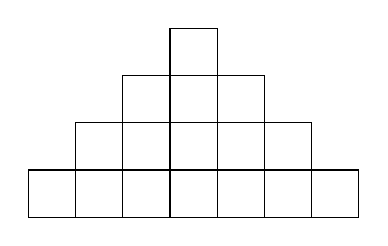
\begin{tikzpicture}[scale=.6]
\draw (0,0)--(7,0);
\draw (0,1)--(7,1);
\draw (1,2)--(6,2);
\draw (2,3)--(5,3);
\draw (3,4)--(4,4);
\foreach \i in {0,...,7}
\draw (\i,0)--(\i,1);
\foreach \i in {1,...,6}
\draw (\i,1)--(\i,2);
\foreach \i in {2,...,5}
\draw (\i,2)--(\i,3);
\foreach \i in {3,...,4}
\draw (\i,3)--(\i,4);
	\end{tikzpicture}
}
\loigiai{
	Số hộp sữa của mỗi hàng lập thành một cấp số cộng với $u_1=1$ và $d=2$.\\
	Theo đề ta có \begin{eqnarray*}
		&&S_n=\dfrac{n[2u_1+(n-1)d]}{2}=900\\&\Leftrightarrow & \dfrac{n[2\cdot 1+(n-1)\cdot 2]}{2}=900\\&\Leftrightarrow & 2n^2=1800\\ &\Leftrightarrow & n^2=900 \\ &\Leftrightarrow &n=30\  (\text{do }n>0).
	\end{eqnarray*}
	Số hộp sữa ở hàng dưới cùng là $u_{30}=1+29\cdot 2=59$.
}
	
\end{ex}
